\documentclass[10pt,twocolumn,letterpaper]{article}

\usepackage{semml}
\usepackage{times}
\usepackage{epsfig}
\usepackage{graphicx}
\usepackage{amsmath}
\usepackage{amssymb}

% Include other packages here, before hyperref.
\usepackage{amsthm}
\usepackage{listings}
\usepackage{braket}
\usepackage{algpseudocodex}
\usepackage{algorithmicx}
\usepackage{multirow}
\usepackage{booktabs}
\usepackage{subcaption}
\usepackage[dvipsnames]{xcolor}
\usepackage{tikz}

% Color scheme
\definecolor{frenchBlue}{HTML}{1C77C3}
\definecolor{razzleDazzleRose}{HTML}{DF57BC}
\definecolor{plum}{HTML}{A03E99}
\definecolor{carrotOrange}{HTML}{F39237}
\definecolor{persianRed}{HTML}{D63230}

% If you comment hyperref and then uncomment it, you should delete
% egpaper.aux before re-running latex.  (Or just hit 'q' on the first latex
% run, let it finish, and you should be clear).
\usepackage[breaklinks=true,bookmarks=false]{hyperref}
\usepackage{lstmisc}

\semmlfinalcopy % *** Uncomment this line for the final submission

\def\semmlPaperID{177} % *** Enter the SemML Paper ID here
\def\httilde{\mbox{\tt\raisebox{-.5ex}{\symbol{126}}}}

% Pages are numbered in submission mode, and unnumbered in camera-ready
%\ifsemmlfinal\pagestyle{empty}\fi
\setcounter{page}{1}
\begin{document}

%%%%%%%%% TITLE
\title{Unsupervised Learning: Improving the K-Means Algorithm}

\author{Juri Kembügler\\
Friedrich-Alexander Universität\\
Erlangen Nürnberg, Germany\\
{\tt\small\href{mailto:juri.kembuegler@fau.de}{juri.kembuegler@fau.de}}
% For a paper whose authors are all at the same institution,
% omit the following lines up until the closing ``}''.
% Additional authors and addresses can be added with ``\and'',
% just like the second author.
% To save space, use either the email address or home page, not both
%\and
%Second Author\\
%Institution2\\
%First line of institution2 address\\
%{\tt\small secondauthor@i2.org}
}

\maketitle
%\thispagestyle{empty}

%%%%%%%%% ABSTRACT
\begin{abstract}
    K-Means is a widely used clustering algorithm, but its effectiveness is often
    limited by poor centroid initialization, leading to suboptimal and unstable
    results. This paper investigates an improved approach proposed by İhsanoğlu and
    Zaval~\cite{Abdullah10601123}, which addresses this issue by identifying and
    correcting conflicting clusters and mega clusters. The method iteratively
    relocates centroids from dense regions to underrepresented areas, refining the
    result without restarting the algorithm. Our experiments on synthetic datasets
    demonstrate that the improved method outperforms both standard K-Means and
    K-Means++ in terms of homogeneity and silhouette scores, while also achieving
    consistent and low-variance convergence across multiple runs.
\end{abstract}

%%%%%%%%% BODY TEXT

\section{Introduction}\label{sec:introduction}

Digitalization has permeated various aspects of our daily lives, from sports
and fitness tracking to video streaming, as well as digital newspaper
consumption. A key consequence of this transformation in recent years is the
vast amount \linebreak of data generated~\cite{Jain2010651}. In 2010, the
global data volume was approximately two zettabytes, whereas by 2024, it had
surged to around 150 zettabytes (1 zettabyte $\approx10^{21}$
bytes)~\cite{IDC_Statista_2024}. Notably, since the onset of the global
COVID-19 pandemic in 2020, the growth rate of data generation and consumption
has accelerated significantly~\cite{IDC_Statista_2024}. Thus, extracting
meaningful insights from this data requires efficient and robust algorithms.

In this context, Machine Learning (ML) has become essential for recognizing
patterns and enabling data-driven decisions. One important branch of ML is
unsupervised learning, where algorithms uncover hidden structures in data
without predefined labels~\cite{deuschle2019}. A fundamental technique in this
domain is clustering, with K-Means being one of the most widely used
methods~\cite{Ezugwu2022104743,Jain2010651}. However, the performance of
K-Means is highly dependent on the initial choice of
centroids~\cite{FRANTI201995,Abdullah10601123}.

\subsubsection{Contributions}

In this article, we make the following contributions: We address K-Means’
sensitivity to centroid initialization by investigating the adjustment strategy
proposed by İhsanoğlu and Zaval~\cite{Abdullah10601123}, which corrects
conflicting and mega clusters through a simple statistical post-processing
step. We formalize the centroid relocation method in clear pseudocode, and
evaluate its effectiveness across four synthetic datasets with varying cluster
separability. Compared to K-Means and K-Means++, the improved approach achieves
consistently higher homogeneity and silhouette scores. It also shows stability
over 1,000 runs, with low variances in clustering results—demonstrating both
improved quality and robustness.

%-------------------------------------------------------------------------

\section{Background and Related Work}\label{sec:background-and-related-work}

%------------------------------------------------------------------------

Clustering is a key technique in unsupervised ML, where the goal is to identify
inherent groupings in data without the use of labelled examples. While
supervised learning relies on input-output pairs to train predictive models,
unsupervised approaches such as clustering work solely with input data to
uncover structure, summarize datasets, or extract meaningful
patterns~\cite{deuschle2019}. This section provides a focused overview of
clustering methods, categorization of clustering algorithms, and the different
types of clusters discussed in prior literature.

\subsection{Clustering}\label{subsec:clustering}

The objective of clustering is to group similar objects based on their
characteristics. The concept of '\textit{similarity}' implies the use of a
distance metric to quantify the relationships between data points. One of the
most widely used distance metrics is the L2 norm (Euclidean
distance)~\cite{deuschle2019}. Alternative metrics such as the L1 norm,
Itakura-Saito or Bregman distance can also be employed, depending on the
specific application and data properties~\cite{Jain2010651}.

Clustering is mainly used to get an overview of data, to summarize it and to
simplify human interpretation by categorizing the data and highlighting
characteristics that distinguish the data points. However, it can also be used
as a preprocessing step for other methods, \eg, feature creation for supervised
learning~\cite{Jain2010651}.

%------------------------------------------------------------------------

\subsubsection{Common clustering algorithms}\label{subsubsec:common-clustering-algorithms}

Overall, clustering algorithms can be classified into two categories:
\textit{hierarchical} and \textit{partitional} algorithms. Hierarchical
algorithms build clusters by recursively merging related data points, whereas
partitional algorithms divide the dataset into distinct clusters
simultaneously~\cite{Ezugwu2022104743,Jain2010651}.

Hierarchical clustering methods include \textit{agglomerative} approaches (such
as single-, complete-, and average-linkage) and \textit{divisive}, \eg,
monothetic and polythetic clustering. Partitional techniques, on the other
hand, encompass algorithms such as \textit{K-Means}, \textit{Genetic
    Algorithms}, \textit{Gaussian Mixture Models}, \textit{Fuzzy C-Means}, and
\textit{DBSCAN}~\cite{Ezugwu2022104743}.

%------------------------------------------------------------------------

\subsection{Types of Clusters}\label{subsec:types-of-clusters}

Kapil Joshi \etal~\cite{Joshi2015} categorize clusters into four distinct
types. In general, the effectiveness of a clustering algorithm heavily depends
on the nature of these underlying structures~\cite{Ezugwu2022104743}. For
instance, density-based algorithms like DBSCAN are particularly effective when
dealing with non-convex cluster shapes~\cite{Bhargav2016}, whereas k-Means
tends to perform best on well-separated, spherical clusters~\cite{Jain2010651}.

According to Kapil Joshi \etal~\cite{Joshi2015}, the four types of clusters are
defined as follows:
\begin{itemize}
    \item\textbf{Well-separated clusters:} A point in a cluster is closer or more similar to any point in the same cluster
          as to a point in another cluster.
          \begin{figure}[h]
              \centering
              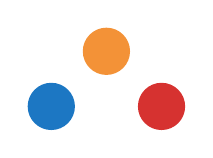
\begin{tikzpicture}
                  % Drei gefüllte Cluster-Kreise
                  \fill[frenchBlue] (-0.7, 0) circle (0.3);
                  \fill[carrotOrange] (0, 0.7) circle (0.3);
                  \fill[persianRed] (0.7, 0) circle (0.3);
              \end{tikzpicture}
              \caption{Well-separated Clusters~\cite{Joshi2015}.}
              \label{fig:well-separated-circles}
          \end{figure}

    \item\textbf{Centre-based clusters:} A point in a cluster is closer or more similar to the ‘centre’ of this cluster
          than to the centre of another cluster.
          \begin{figure}[h]
              \centering
              
\begin{tikzpicture}
                  \fill[frenchBlue] (0,0) circle (0.3);
                  \fill[carrotOrange] (0.6,0.2) circle (0.3);
                  \fill[persianRed] (1.8,0) circle (0.3);
                  \fill[plum] (2.3,0.1) circle (0.3);
              \end{tikzpicture}
              \caption{Centre-based clusters~\cite{Joshi2015}.}
              \label{fig:well-separated}
          \end{figure}

    \item\textbf{Contiguous clusters:} A point in a cluster is closer to one or more points in the same cluster as to
          any other point not in the cluster.
          \begin{figure}[h]
              \centering
              
\includegraphics[width=0.5\linewidth]{figures/Contigous clusters}
              \caption{Contiguous clusters~\cite{Joshi2015}.}
              \label{fig:Contiguous-clusters}
          \end{figure}

    \item\textbf{Density-based clusters:} A cluster is a dense region of points separated from other high-density
          regions by low-density regions.
          \begin{figure}[h]
              \centering
              
\includegraphics[width=0.5\linewidth]{figures/Density-based clusters}
              \caption{Density-based clusters~\cite{Joshi2015}.}
              \label{fig:density-based-clusters}
          \end{figure}
\end{itemize}

%------------------------------------------------------------------------

\section{K-Means}\label{sec:k-means}

This section introduces the K-Means clustering algorithm, detailing its
historical origins and general procedure. We then focus on Lloyd’s algorithm,
the most common implementation, and explain its iterative optimization steps.
The limitations of K-Means are discussed, including challenges in choosing the
number of clusters and initializing centroids. Finally, we present the
K-Means++ algorithm, a widely used technique to improve centroid
initialization.

\subsection{Background and Procedure}\label{subsec:background-and-procedure}

In contrast to other algorithms, K-Means was discovered independently in
various research fields, first by Steinhaus (1956) and Lloyd (proposed 1957;
published 1982) and later by Ball and Hall (1965) and MacQueen
(1967)~\cite{Jain2010651}.

Despite variations in their implementation, all K-Means algorithms follow the
same fundamental procedure for partitioning data into clusters. Given an input
dataset represented as a $n \times d$ matrix—where $n$ is the number of data
points and $d$ the number of features—K-Means requires the number of desired
clusters, a similarity metric and an initialization strategy. The core
algorithm, illustrated in Fig.~\ref{fig:kmeans-procedure}, proceeds as follows:
\begin{algorithmic}[1]
    \Require $X$, $k$, similarity metric, initialization strategy
    \State Initialize $k$ centroids $\mu_{1, \dots, k}$ using the chosen strategy
    \Repeat
    \For{each $x_i \in X$}
    \State Assign $x_i$ to the cluster with the nearest centroid based on the similarity metric
    \EndFor
    \For{each cluster $j = 1$ to $k$}
    \State $\mu_j\gets$ mean of all $x$ assigned to cluster $j$
    \EndFor
    \Until{no data point changes its assigned cluster}
\end{algorithmic}
While the pseudocode above reflects the standard implementation, they differ subtly in their objectives and
approaches. For example, unlike Lloyd's algorithm, which updates centroids only
after all data points have been reassigned, MacQueen's algorithm performs
incremental updates, adjusting the affected cluster’s centroid immediately when
a data point moves from one cluster to another~\cite{Morissette2013}.

\begin{figure}[h]
    \centering
    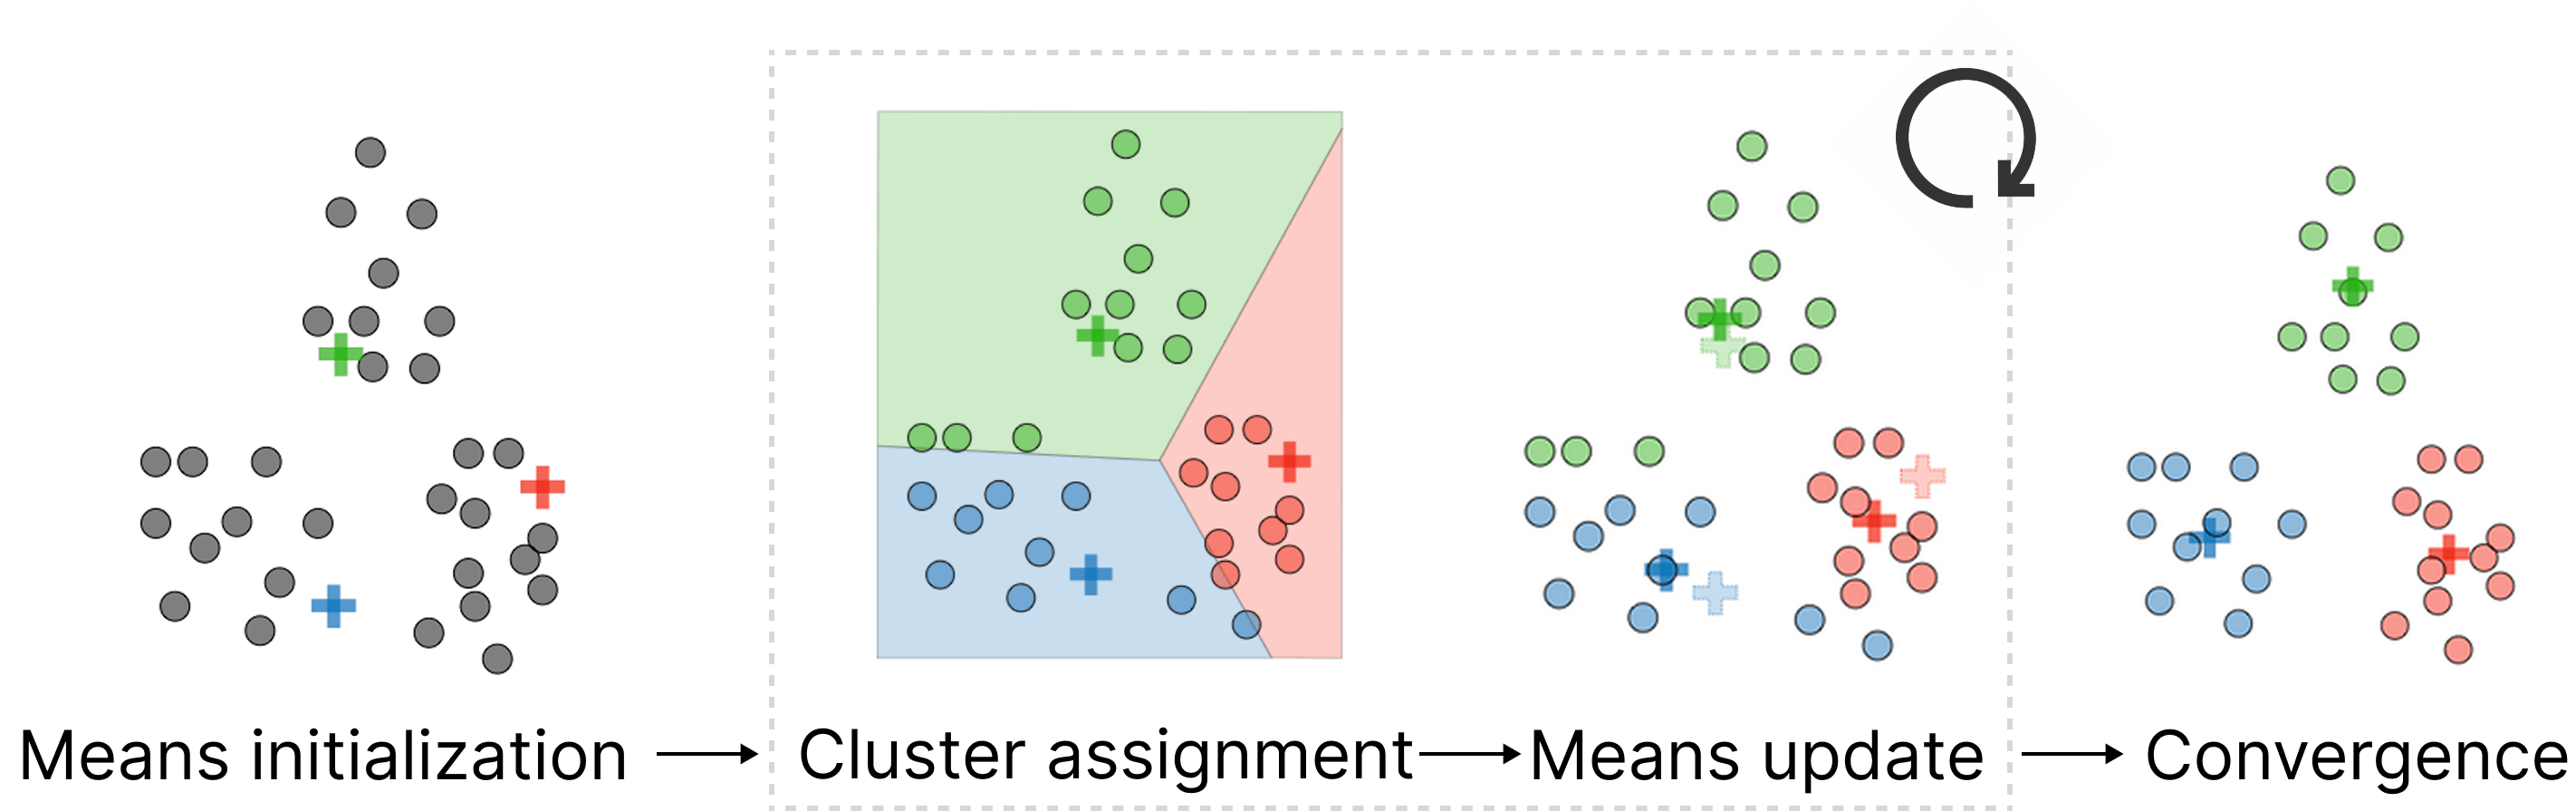
\includegraphics[width=1\linewidth]{figures/K-Means procedure}
    \caption{K-Means procedure visualized \cite{Amidi2018}.}
    \label{fig:kmeans-procedure}
\end{figure}

%------------------------------------------------------------------------

\subsection{Lloyd's algorithm}\label{subsec:procedure-and-lloyd's-algorithm}

One of the most widely used implementations of K-Means is Lloyd’s
algorithm~\cite{deuschle2019}, which iteratively refines cluster assignments
and centroids through a simple yet effective approach. Given a dataset
$X=\set{x_i}_{i=1}^N$ of $d$-dimensional points, the goal is to iteratively
refine the centroids $C=\Set{\mu_i}_{i=1}^k$ to partition the data into $k$
clusters. The assignment of data points to clusters is encoded by a
responsibility vector $R\in\Set{0,1}^{N\times k}$, where $r_{nk}=1$ indicates
that point $x_n$ belongs to cluster $k$, and $0$ otherwise.

To quantify clustering quality, we define the loss function, also known as the
\textit{sum-of-squared errors (SSE)}, as the sum of squared distances between
data points and their assigned centroids:
\begin{equation}
    \label{eq:lloyds-loss}
    \mathcal{L} = \sum_{n=1}^{N} \sum_{c=1}^{k} r_{nc} \|x_n - \mu_c\|^2.
\end{equation}
To minimize the loss $\mathcal{L}$, Lloyd's algorithm iterates between two steps~\cite{deuschle2019, FRANTI201995}:
\begin{enumerate}
    \item \textbf{Assignment Step:} Each data point is assigned to the nearest centroid by updating the responsibility vector:
          \begin{equation}
              \label{eq:lloyds-res-vec}
              r_{nc} =
              \begin{cases}
                  1, & \text{if } c = \underset{c'}{\arg\min} \|x_n - \mu_{c'}\| \\
                  0, & \text{otherwise.}
              \end{cases}
          \end{equation}
    \item \textbf{Update Step:} The cluster centroids are recomputed as the mean of all assigned points:
          \begin{equation}
              \label{eq:min-lloyds-loss}
              \mu_c' = \frac{\sum_{n=1}^{N} r_{nc} x_n}{\sum_{n=1}^{N} r_{nc}}.
          \end{equation}
\end{enumerate}
These steps repeat until the assignments $R$ no longer change, indicating
convergence. Since the loss function $\mathcal{L}$ is non-increasing at each
iteration, the algorithm is guaranteed to reach a local minimum, though not
necessarily the global optimum.

%------------------------------------------------------------------------

\subsection{Problems and limitations}\label{subsec:problems-and-limitations}

Despite its simplicity and efficiency, K-Means has several
limitations~\cite{Ezugwu2022104743, FRANTI201995, Jain2010651}. Since it relies
on distance calculations, standardizing data is often necessary to ensure equal
feature contributions~\cite{Morissette2013}. The algorithm’s sensitivity to the
choice of $k$ and centroid initialization can significantly impact performance.
This section explores these challenges and strategies to address them.

%------------------------------------------------------------------------

\subsubsection{Choose $k$}

One of the few adjustable parameters in Lloyd's algorithm, apart from the
initialization method, is the number of clusters $k$. Examining the loss
function in Equation~(\ref{eq:lloyds-loss}), we observe that a smaller number
of clusters generally results in a higher loss, as data points are assigned to
fewer centroids. Conversely, the loss decreases as $k$ increases, reaching its
minimum when each data point forms its own cluster. However, this solution is
not meaningful, as it eliminates the concept of clustering altogether
~\cite{deuschle2019}. Since there is no optimal choice for $k$,
Jain~\cite{Jain2010651} suggests running the algorithm with multiple values of
$k$ and selecting the most significant one based on evaluation criteria.

A widely used heuristic for determining $k$ is the \textit{elbow method}. This
approach involves plotting the loss function against $k$ and identifying the
point where the decrease in loss slows significantly—forming an
'\textit{elbow}' in the curve (see Fig.~\ref{fig:elbow-plot}). The fundamental
concept behind this method is that above a certain $k$, additional clusters
result in diminishing returns in loss reduction~\cite{deuschle2019}.

\begin{figure}[t]
    \centering
    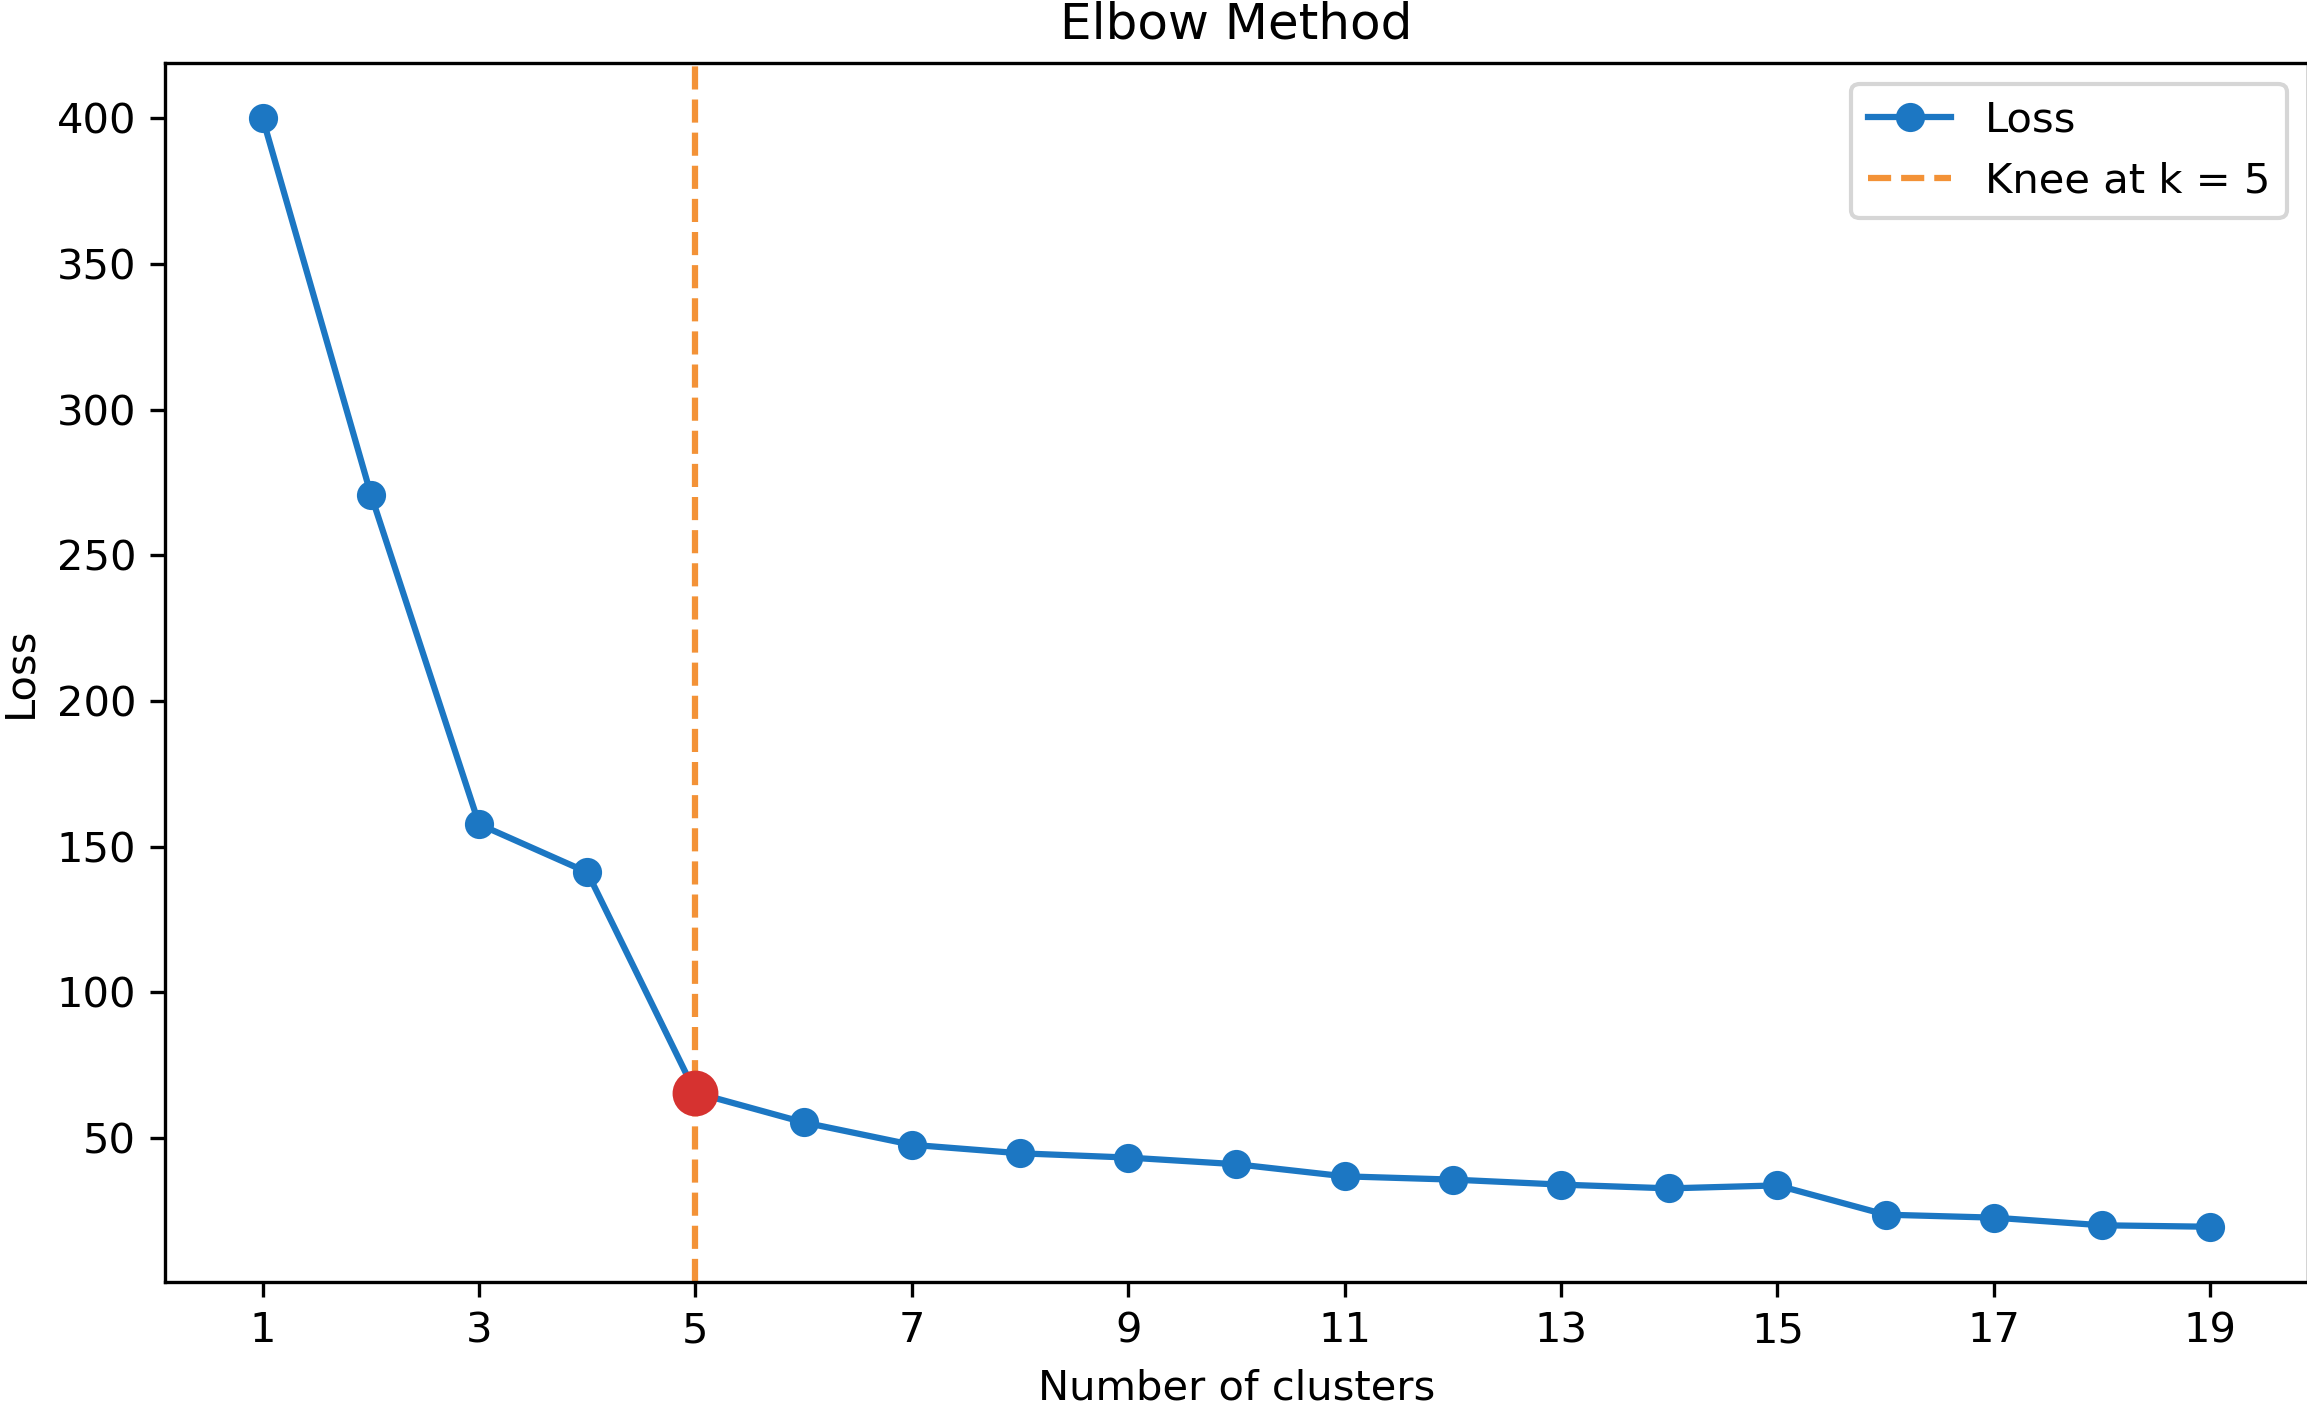
\includegraphics[width=0.9\linewidth]{figures/elbow_method}
    \caption{Elbow plot using the Mall Customer Segmentation Data~\cite{KaggleMallDataset}.}
    \label{fig:elbow-plot}
\end{figure}

%------------------------------------------------------------------------

\subsubsection{Centroid initialization}

The simplest method for initializing centroids is to select them randomly.
However, as previously discussed, Lloyd’s algorithm converges to a local
minimum, making the final clustering outcome highly sensitive to the initial
centroid selection. Consequently, poor initialization can lead to suboptimal
solutions~\cite{FRANTI201995,Abdullah10601123}.

According to Fränti and Sieranoja~\cite{FRANTI201995}, there are two main ways
to mitigate K-Means’ sensitivity to centroid initialization: (1) using improved
initialization techniques and (2) running the algorithm multiple times and
selecting the best result based on a predefined criterion. Several heuristics
have been proposed to enhance initialization:
\begin{itemize}
    \item \textbf{Random points:} Centroids are chosen randomly from the dataset.
    \item \textbf{Furthest point heuristic:} The first centroid is chosen randomly, and subsequent centroids are selected to be as far as possible from those already chosen.
    \item \textbf{Sorting heuristic:} Data points are sorted by a criterion, \eg, projection along a principal component and used for initialization.
    \item \textbf{Density-based:} This method selects centroids in high-density regions.
    \item \textbf{Projection-based:} A dimensionality reduction technique identifies representative points for initialization.
    \item \textbf{Splitting technique:} A small number of centroids are initialized first, then iteratively refined by splitting.
\end{itemize}
Despite these efforts, \textit{"a clear state-of-the-art is
    missing"}~\cite{FRANTI201995}, meaning no single method consistently
outperforms others across all datasets. However, one widely adopted
initialization method is K-Means++, which balances randomness with a
distance-based heuristic to improve clustering performance.

%------------------------------------------------------------------------

\subsection{K-Means++}\label{subsec:k-means++}

As previously discussed, K-Means is highly sensitive to the initial choice of
centroids. K-Means++ is a popular initialization strategy designed to mitigate
this issue by selecting centroids in a more systematic manner. The algorithm,
outlined in the following pseudocode, proceeds as follows:
\begin{algorithmic}[1]
    \Require $X$, $k$
    \State Randomly select the first centroid $\mu_1$ from $X$
    \For{$i = 2$ to $k$}
    \State Compute the distance $D_j=d(x_j, \mu_{\text{neigh}})$ from each $x_j\in X$ to the nearest centroid $\mu_{\text{neigh}}$
    \State Select the next centroid $\mu_i$ with probability proportional to ${D_j}^2$
    \EndFor
\end{algorithmic}
K-Means++ generally improves clustering performance by offering more effective
initial centroid placement~\cite{FRANTI201995}. Nevertheless, due to its
randomness, it does not entirely eliminate the risk of converging to
suboptimal solutions~\cite{deuschle2019, Abdullah10601123}.

%------------------------------------------------------------------------

\section{Statistically improving K-Means}\label{sec:statistically-improving-k-means}

As noted by Fränti and Sieranoja~\cite{FRANTI201995}, K-Means presents several
opportunities for optimization. However, a key limitation is that centroids
struggle to relocate effectively when they are initially placed far from their
optimal positions. To address this issue, İhsanoğlu and
Zaval~\cite{Abdullah10601123} propose an initial solution based on simple
statistical methods, facilitating more efficient centroid movement.

%------------------------------------------------------------------------

\subsection{Identifying issues}\label{subsec:identifying-issues}

As previously mentioned, one of the main challenges in K-Means is that poorly
initialized centroids may struggle to reach their optimal positions, if at all.
This often leads to an uneven distribution of centroids—some regions may
contain too many, while others are underrepresented~\cite{FRANTI201995}. In
order to characterize such imbalances, İhsanoğlu and
Zaval~\cite{Abdullah10601123} propose separate approaches for
\textit{conflicting clusters} and \textit{mega clusters}.

\subsubsection{Conflicting Clusters}

This type of cluster arises when multiple centroids are located too close to
one another, typically indicating redundant clustering in a dense region. To
detect them, we first compute the average distance between each centroid and
its nearest neighbour:
\begin{equation}
    \label{eq:avgDist}
    \text{AvgDist} = \frac{1}{k} \sum_{i=1}^{k} d(\mu_i, \mu_{\text{neigh}}).
\end{equation}
Where $k$ is the number of clusters, $d(x,y)$ is the distance function, \eg, Euclidean, and $\mu_{\text{neigh}}$ denotes the closest centroid to $\mu_i$.
Using this average, we define a threshold by introducing a tunable
hyperparameter $t$. Any pair of centroids closer than $\text{AvgDist} / t$ is
considered a conflicting cluster:
\begin{equation}
    \label{eq:conflicting-cluster}
    C_i \text{ is conflicting} \iff d(\mu_i, \mu_{\text{neigh}}) < \frac{\text{AvgDist}}{t}.
\end{equation}

\subsubsection{Mega Clusters}

When too few centroids are assigned to a region, this can lead to the formation
of large, coarse-grained clusters. These \textit{mega clusters} often encompass
multiple natural groupings. To detect them, we first calculate the
intra-cluster variance:
\begin{equation}
    \label{eq:cluster-var}
    \text{Var}(C_i) = \frac{1}{\sum_{n=1}^{N} (r_{ni}) - 1} \sum_{n=1}^{N} r_{ni} \|x_n - \mu_i\|^2.
\end{equation}
Here, $r_{ni}$ indicates cluster membership, and $\|x_n - \mu_i\|^2$ measures
the squared distance from the data point to the cluster centroid. The mega
cluster is then defined as the cluster with the highest variance:
\begin{equation}
    \label{eq:mega-cluster}
    C_{\max} = \underset{C_i}{\arg\max}\text{ Var}(C_i).
\end{equation}

%------------------------------------------------------------------------

\subsection{The improved algorithm}\label{subsec:the-improved-algorithm}

Based on the previously defined concepts of conflicting and mega clusters,
İhsanoğlu and Zaval~\cite{Abdullah10601123} propose an extension to K-Means
that iteratively relocates redundant centroids. The procedure is as follows:
run K-Means (or K-Means++) as usual, identify conflicting and mega clusters,
then iteratively move a centroid from a conflicting cluster to a randomly
chosen point in the mega cluster. This process is repeated until no conflicting
clusters remain or a maximum number of iterations is reached.

This post-processing strategy refines the clustering outcome without re-running
the full algorithm, making it computationally efficient, compared to current
solutions. By relocating centroids from overcrowded to underrepresented
regions, the method directly addresses initialization-induced imbalance.
Although conceptually simple, it was shown by İhsanoğlu and Zaval to enhance
cluster separation and compactness across a range of datasets. The pseudocode
below summarizes the method:

\begin{algorithmic}[1]
    \label{alg:imprv-kmeans}
    \Require $X$, $k$, init\_func, max\_iter $ \in \mathbb{N}$, $t \in [1, \infty)$
    \State $C \gets$ \texttt{init\_func}$(X, k)$
    \State
    \For{$i = 1$ To $max\_iter$}
    \State $C,R \gets$ \texttt{converge\_to\_clusters}$(C, X, k)$
    \State
    \State $conflicts \gets$ \texttt{Get\_conflicts}$(C, t)$
    \State
    \If{\texttt{len}$(conflicts) = 0$}
    \State \textbf{break}
    \EndIf
    \State
    \State $mega\_cl \gets$ \texttt{Get\_mega\_cluster}$(X, k, R)$
    \State
    \State $conflict \gets$ \texttt{rand.choice}$(conflicts)$
    \State $C[conflict] \gets$ \texttt{rand.choice}$(mega\_cl)$
    \EndFor
    \State \Return $C,~R$
\end{algorithmic}

%------------------------------------------------------------------------

\begin{table*}
    \centering
    \begin{tabular}{ll c c c c c c}
        \toprule
                                             &                  & \multicolumn{2}{c}{\textbf{K-Means}} & \multicolumn{2}{c}{\textbf{K-Means++}} & \multicolumn{2}{c}{\textbf{Improved}}                                                              \\
        \cmidrule(lr){3-4} \cmidrule(lr){5-6} \cmidrule(lr){7-8}
                                             &                  & \textbf{Score}                       & \textbf{Variance}                      & \textbf{Score}                        & \textbf{Variance} & \textbf{Score}  & \textbf{Variance}    \\
        \midrule
        \multirow{2}{*}{\textbf{S1-Dataset}} & \textbf{H-Score} & 0.9209                               & 0.0008                                 & 0.9504                                & 0.0006            & \textbf{0.9863} & $\mathbf{\approx 0}$ \\
                                             & \textbf{S-Score} & 0.6121                               & 0.0017                                 & 0.6540                                & 0.0015            & \textbf{0.7113} & $\mathbf{\approx 0}$ \\
        \midrule
        \multirow{2}{*}{\textbf{S3-Dataset}} & \textbf{H-Score} & 0.7656                               & 0.0003                                 & 0.7701                                & 0.0003            & \textbf{0.7941} & $\mathbf{\approx 0}$ \\
                                             & \textbf{S-Score} & 0.4609                               & 0.0003                                 & 0.4642                                & 0.0003            & \textbf{0.4915} & $\mathbf{\approx 0}$ \\
        \midrule
        \multirow{2}{*}{\textbf{A1-Dataset}} & \textbf{H-Score} & 0.9181                               & 0.0010                                 & 0.9492                                & 0.0006            & \textbf{0.9978} & $\mathbf{\approx 0}$ \\
                                             & \textbf{S-Score} & 0.5162                               & 0.0009                                 & 0.5454                                & 0.0006            & \textbf{0.5951} & $\mathbf{\approx 0}$ \\
        \midrule
        \multirow{2}{*}{\textbf{A3-Dataset}} & \textbf{H-Score} & 0.9360                               & 0.0002                                 & 0.9587                                & 0.0001            & \textbf{0.9982} & $\mathbf{\approx 0}$ \\
                                             & \textbf{S-Score} & 0.5160                               & 0.0004                                 & 0.5439                                & 0.0003            & \textbf{0.5999} & $\mathbf{\approx 0}$ \\
        \bottomrule
    \end{tabular}
    \vspace{5pt}
    \caption{
        Clustering performance on four synthetic datasets~\cite{ClusteringDatasets}, evaluated using Homogeneity (H-Score) and Silhouette (S-Score). Each method was run 1,000 times; mean and variance are reported. The improved method shows consistently higher scores and near-zero (below $10^{-4}$) variances, indicating stable convergence. The data is publicly available here: \href{https://cs.uef.fi/sipu/datasets/}{https://cs.uef.fi/sipu/datasets/}.
    }
    \label{tab:clustering_comparison}
\end{table*}

%------------------------------------------------------------------------

\subsection{Challenges}\label{subsec:challenges}

While the improved method introduces additional statistical computations and
iterations, it differs from traditional approaches in that it does not restart
the entire clustering process. Instead, it incrementally refines an initial
K-Means result~\cite{Abdullah10601123}. This targeted adjustment increases the
likelihood of escaping poor local minima and reaching a more optimal clustering
configuration—something that is often challenging to achieve through multiple
K-Means runs alone~\cite{FRANTI201995}.

A key limitation of the approach is its dependence on the choice of the
threshold parameter~$t$. To ensure meaningful identification of conflicting
clusters, $t$ must satisfy $t > 1$; otherwise, nearly all clusters would be
classified as conflicting. Conversely, if $t$ is set too high, the algorithm
may terminate prematurely without any adjustments.

One potential strategy is to begin with a small value of $t$ and incrementally
increase it until convergence is achieved before reaching the maximum number of
iterations. However, this introduces ambiguity: Early convergence could either
indicate a well-chosen threshold or that K-Means had already produced a
near-optimal solution, making it difficult to assess the effectiveness of $t$
in isolation.

%------------------------------------------------------------------------

\section{Results and Performance Evaluation}\label{sec:results-and-performance-evaluation}

We evaluate the improved clustering algorithm against K-Means and K-Means++
using synthetic datasets, focusing on clustering quality and stability.
Performance is measured with homogeneity and silhouette scores over several
independent runs to assess both accuracy and consistency.

%------------------------------------------------------------------------

\subsection{Methodology}\label{subsec:methodology}

To ensure reliable results, we conduct $1,000$ independent runs of each
algorithm across multiple datasets. The performance of the algorithms is
measured using two common clustering evaluation metrics: homogeneity and
silhouette score. For each dataset, we compute the mean and variance of these
scores to assess both the quality and stability of the clustering results.

\subsubsection{Datasets}

The following synthetic datasets, as introduced in~\cite{ClusteringDatasets},
are used to evaluate clustering performance:

\begin{itemize}
    \item \textbf{A-Sets:} Artificial datasets with a large number of well-separated clusters. They test the algorithm’s ability to accurately partition clearly defined groups.
    \item \textbf{S-Sets:} Synthetic datasets characterized by overlapping or closely spaced clusters. These challenge the algorithm’s precision in distinguishing densely packed data.
\end{itemize}
Together, these datasets provide a set of
diverse and complementary perspectives on clustering
quality under varying structural conditions.

\subsubsection{Metrics}

To assess the quality of the clustering results, we employ the following used
evaluation metrics~\cite{Abdullah10601123}:

\begin{itemize}
    \item \textbf{Homogeneity Score:} This metric evaluates whether each cluster contains only data points from a single ground truth class. A score of $1.0$ indicates perfectly homogeneous clusters.
    \item \textbf{Silhouette Score:} This metric measures how well each data point matches to its own cluster compared to other clusters. It evaluates the extent to which a data point is closer to points within its own cluster than to points in other clusters. The score ranges from $-1$ to $1$, with higher values indicating that data points are well-clustered, meaning they are both tightly grouped within their cluster and distinct from points in other clusters.
\end{itemize}

%------------------------------------------------------------------------

\subsection{Measurement results}\label{subsec:measurement-results}

Table~\ref{tab:clustering_comparison} presents the clustering performance of
the three algorithms—K-Means, K-Means++, and the improved method—on two
synthetic datasets: \textit{S1} and \textit{A1}. Each algorithm was evaluated
using the Homogeneity Score (H-Score) and Silhouette Score (S-Score), along
with their respective variances, based on 1,000 independent runs.

Across both datasets and metrics, the improved method consistently outperforms
K-Means and K-Means++ in terms of both mean score and stability. Notably, the
variance for the improved method is below $10^{-4}$ in all cases, indicating
consistency in its clustering results. This reflects the algorithm’s robustness
in overcoming initialization sensitivity, a common issue in K-Means-based
approaches.

For example, on the S1 dataset, the improved algorithm achieves an H-Score of
0.9863 and an S-Score of 0.7113, surpassing K-Means++ (0.9504 and 0.6540,
respectively) and K-Means (0.9209 and 0.6121). A similar pattern is observed in
the A3 dataset, where the improved approach again reaches near-perfect
homogeneity and the highest silhouette value.

These results demonstrate the effectiveness of the conflict resolution and
redistribution strategy in enhancing both clustering accuracy and reliability.

%------------------------------------------------------------------------

\section{Conclusion}\label{sec:conclusion}

In this paper, we revisited the well-known K-Means algorithm and highlighted a
central issue: its tendency to become stuck in suboptimal configurations due to
poorly initialized centroids. Building on İhsanoğlu and Zaval’s method
~\cite{Abdullah10601123}, we implemented the enhancement that iteratively
relocates centroids from densely populated regions (conflicting clusters) to
underrepresented ones (mega clusters), leading to improvements in clustering
performance and stability.

Our evaluation across multiple synthetic datasets shows that the approach
consistently outperforms both K-Means and K-Means++ in terms of homogeneity and
silhouette scores. Moreover, the method achieves low variance in repeated runs,
suggesting robust and reliable behaviour.

While the method introduces a new hyperparameter $t$, we discussed its
influence and outlined basic strategies for its selection. Although further
evaluation on real-world datasets is required, the approach provides a
lightweight refinement step that can improve K-Means results without fully
reinitializing the algorithm.

Future work could explore adaptive threshold tuning and application to
high-dimensional or real-world datasets.

    %-----------------------------------------------------------------------

    %------------------------------------------------------------------------

    {\small
        \bibliographystyle{ieee}
        \bibliography{kembuegler_bib}
    }

\end{document}
